\documentclass{article}
\usepackage[paperwidth=3.45in,paperheight=3.80in,margin=0pt]{geometry}
% CN: 与 icml2026.sty 一致，仅使用 Times 正文字体，保留默认数学字体及 mathcal。
% EN: Match icml2026.sty: Times text with the default math fonts and mathcal alphabet.
\usepackage{times}
\usepackage{courier}
\usepackage{amsmath,amssymb}
\usepackage{tikz}
\usetikzlibrary{arrows.meta,calc,decorations.pathreplacing}
\pagestyle{empty}
\setlength{\parindent}{0pt}

% CN: 独立编译，保持单栏宽度；纵向比例接近已审核的概览草图。
% EN: Compile independently at native column width; retain the approved portrait composition.
% CN: 颜色对应 paper_experiments/palettes.json 的 scientific 语义角色。
% EN: Colors map to scientific semantic roles in paper_experiments/palettes.json.
\definecolor{proposed}{HTML}{EE6A5F}
\definecolor{inherited}{HTML}{4E79A7}
\definecolor{support}{HTML}{86B7B2}
\definecolor{accent}{HTML}{F2C75E}
\definecolor{candidate}{HTML}{F4A261}
\definecolor{ink}{HTML}{3D3D3A}
\colorlet{border}{ink!55}
\colorlet{initialarrow}{inherited!70!white}
\colorlet{operatorink}{inherited!85!ink}

\newcommand{\op}[1]{\textcolor{operatorink}{\texttt{\bfseries #1}}}
\newcommand{\smalltype}{\fontsize{7.2}{8.3}\selectfont}
\newcommand{\basetype}{\fontsize{8.5}{9.5}\selectfont}
\newcommand{\titletype}{\fontsize{9}{10}\selectfont\bfseries}

% CN: 标题带裁剪在圆角面板内；位置与大小独立于文字长度。
% EN: Header bands are clipped to rounded panels; geometry is independent of text lengths.
\newcommand{\headedpanel}[5]{%
  \begin{scope}
    \clip[rounded corners=1.4mm] (#1,#2) rectangle (#3,#4);
    \fill[ink!6] (#1,#4-5.5) rectangle (#3,#4);
  \end{scope}
  \draw[panel] (#1,#2) rectangle (#3,#4);
  \node[heading] at (#1+1.7,#4-2.75) {#5};}

% CN: support 表示允许的变量；state 的填色表示正流量，空白表示零流量。
% EN: Support marks allowed variables; filled state cells denote positive flow and blank cells denote zero flow.
\newcommand{\supportglyph}[2]{%
  \begin{scope}[shift={(#1,#2)}]
    \foreach \i/\j in {0/4,3/4,1/3,0/2,4/2,2/1,3/0}
      \fill[support!75] (2.5*\i,2.5*\j) rectangle ++(2.5,2.5);
    \draw[step=2.5,draw=ink!75,line width=.4pt] (0,0) grid (12.5,12.5);
    \draw[draw=ink!90,line width=.7pt] (0,0) rectangle (12.5,12.5);
  \end{scope}}

\newcommand{\stateglyph}[2]{%
  \begin{scope}[shift={(#1,#2)}]
    \foreach \i/\j in {0/4,1/3,4/2,2/1,3/0}
      \fill[support!75] (2.5*\i,2.5*\j) rectangle ++(2.5,2.5);
    \draw[step=2.5,draw=ink!75,line width=.4pt] (0,0) grid (12.5,12.5);
    \draw[draw=ink!90,line width=.7pt] (0,0) rectangle (12.5,12.5);
    \foreach \k in {0,...,4} {
      \filldraw[fill=proposed!48,draw=ink!65,line width=.4pt]
        (-2.8,2.5*\k) rectangle ++(1.9,2.5);
      \filldraw[fill=accent!65,draw=ink!65,line width=.4pt]
        (2.5*\k,13.5) rectangle ++(2.5,1.9);
    }
    \node[inner sep=0pt] at (-4.4,6.25) {$f$};
    \node[inner sep=0pt] at (-1,14.45) {$g$};
  \end{scope}}

\begin{document}
\noindent
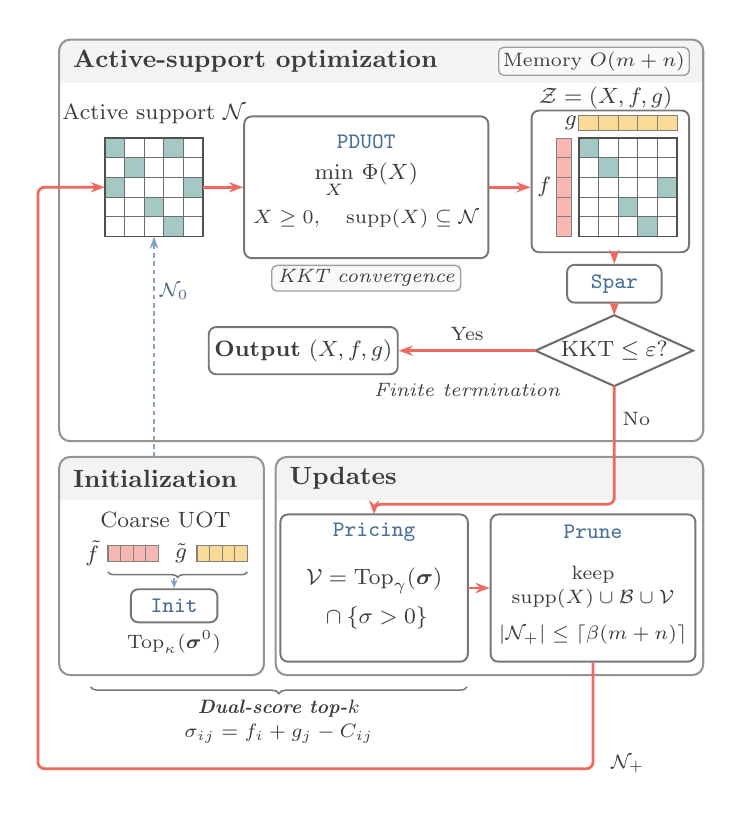
\begin{tikzpicture}[
  x=1mm,y=1mm,font=\basetype,text=ink,
  panel/.style={draw=border,rounded corners=1.4mm,line width=.75pt},
  box/.style={draw=ink!70,rounded corners=.95mm,line width=.7pt,fill=white,inner sep=0pt,align=center},
  pill/.style={draw=ink!50,rounded corners=.65mm,line width=.5pt,fill=ink!3,inner sep=.55mm,font=\smalltype},
  mainarrow/.style={-{Stealth[length=1.8mm,width=1.3mm]},draw=proposed,line width=1pt,rounded corners=.85mm},
  initarrow/.style={-{Stealth[length=1.55mm,width=1.1mm]},draw=initialarrow,line width=.7pt,dash pattern=on 1.7pt off 1.3pt,rounded corners=.85mm},
  heading/.style={font=\titletype,anchor=west,inner sep=0pt}
]
\path[use as bounding box] (0,0) rectangle (87.63,96.52);

% CN: 上部主循环保留参考图的标题带、求解器、state 外框和输出分支。
% EN: The main loop retains the reference's header band, solver, framed state and output branch.
\headedpanel{4}{44}{85.8}{95}{Active-support optimization}
\node[pill,anchor=east] at (84.1,92.25) {Memory $O(m+n)$};

\node[inner sep=0pt] at (16.05,85.5) {Active support $\mathcal N$};
\supportglyph{9.8}{70}
\node[box,minimum width=31mm,minimum height=18mm] (solver) at (43,76.25) {};
\node at (43,82) {\op{PDUOT}};
\node at (43,77.1) {$\min\limits_X\,\Phi(X)$};
\node[font=\smalltype] at (43,72.3) {$X\geq0,\quad\operatorname{supp}(X)\subseteq\mathcal N$};
\node[pill,font=\smalltype\itshape,minimum width=24mm] at (43,64.7) {KKT convergence};

\node[box,minimum width=20mm,minimum height=18mm] (state) at (74,77) {};
\stateglyph{70}{70}
\node[inner sep=0pt] at (73.4,87.6) {$\mathcal Z=(X,f,g)$};
\node[box,minimum width=12mm,minimum height=4.8mm] (spar) at (74.5,64) {\op{Spar}};
\coordinate (checknorth) at (74.5,60);
\coordinate (checksouth) at (74.5,51);
\coordinate (checkwest) at (64.5,55.5);
\draw[draw=ink!75,line width=.75pt,fill=white]
  (checknorth) -- (84.5,55.5) -- (checksouth) -- (checkwest) -- cycle;
\node[inner sep=0pt] at (74.5,55.5) {$\mathrm{KKT}\leq\varepsilon$?};
\node[box,minimum width=24mm,minimum height=6mm] (output) at (35,55.5)
  {\textbf{Output} $(X,f,g)$};

\draw[mainarrow] (22.3,76.25) -- (solver.west);
\draw[mainarrow] (solver.east) -- (state.west |- solver.center);
\draw[mainarrow] (74.5,68) -- (spar.north);
\draw[mainarrow] (spar.south) -- (checknorth);
\draw[mainarrow] (checkwest) -- node[above,font=\smalltype,text=ink] {Yes} (output.east);
\node[font=\smalltype\itshape] at (55.8,50.5) {Finite termination};

% CN: 下部保留两个同级标题，Pricing 与 Prune 具有独立卡片。
% EN: The lower modules have peer headings, with separate Pricing and Prune cards.
\headedpanel{4}{14.3}{30}{42}{Initialization}
\headedpanel{31.5}{14.3}{85.8}{42}{Updates}
\node[inner sep=0pt] at (17.5,34) {Coarse UOT};

% CN: 两组对偶向量横向并排，给下方 Init 与选择公式留出间距。
% EN: Two horizontal dual vectors leave room below for Init and its selection formula.
\foreach \k in {0,...,3} {
  \filldraw[fill=proposed!48,draw=ink!65,line width=.4pt]
    (10.2+1.6*\k,28.7) rectangle ++(1.6,2.1);
  \filldraw[fill=accent!65,draw=ink!65,line width=.4pt]
    (21.5+1.6*\k,28.7) rectangle ++(1.6,2.1);
}
\node[inner sep=0pt] at (8.2,29.75) {$\tilde f$};
\node[inner sep=0pt] at (19.5,29.75) {$\tilde g$};
\draw[decorate,decoration={brace,mirror,amplitude=.7mm},draw=ink!70,line width=.55pt]
  (10.2,27.4) -- (27.9,27.4);
\node[box,minimum width=11mm,minimum height=4.2mm] (init) at (18.6,23.1)
  {\textcolor{inherited!80!ink}{\texttt{\bfseries Init}}};
\draw[-{Stealth[length=1.1mm,width=.85mm]},draw=initialarrow,line width=.65pt]
  (18.6,26.6) -- (init.north);
\node[font=\smalltype,inner sep=0pt] at (18.6,18.5)
  {$\operatorname{Top}_{\kappa}(\boldsymbol\sigma^0)$};

\node[box,minimum width=23.8mm,minimum height=18.7mm] (pricingcard) at (44,25.35) {};
\node at (44,32.5) {\op{Pricing}};
\node[inner sep=0pt,align=center] at (44,24)
  {$\begin{gathered}\mathcal V=\operatorname{Top}_{\gamma}(\boldsymbol\sigma)\\
    {}\cap\{\sigma>0\}\end{gathered}$};
\node[box,minimum width=26mm,minimum height=18.7mm] (prune) at (71.8,25.35) {};
\node at (71.8,32.5) {\op{Prune}};
\node[font=\smalltype] at (71.8,27) {keep};
\node[font=\smalltype] at (71.8,24) {$\operatorname{supp}(X)\cup\mathcal B\cup\mathcal V$};
\node[font=\smalltype] at (71.8,19.4) {$|\mathcal N_+|\leq\lceil\beta(m+n)\rceil$};

% CN: 细括线仅关联 Init 与 Pricing 的共用规则，不表示控制流。
% EN: The light brace links the shared Init/Pricing rule without representing control flow.
\draw[decorate,decoration={brace,mirror,amplitude=.85mm},draw=ink!70,line width=.55pt]
  (8,12.8) -- (55.8,12.8);
\node[font=\smalltype\bfseries\itshape] at (31.9,10) {Dual-score top-$k$};
\node[font=\smalltype] at (31.9,6.9) {$\sigma_{ij}=f_i+g_j-C_{ij}$};

% CN: 主循环单线闭合，初始化独立入场；连线均避开标题和正文。
% EN: One closed path forms the main loop; initialization enters separately, avoiding labels.
\draw[mainarrow] (checksouth) -- (74.5,36) -- (44,36) -- (44,34.7);
\node[font=\smalltype,anchor=west,inner sep=0pt] at (75.5,46.9) {No};
\draw[mainarrow] (55.9,25.35) -- (prune.west);
\draw[mainarrow] (prune.south) -- (71.8,2.4)
  -- (1.3,2.4) -- (1.3,76.25) -- (9.8,76.25);
\node[font=\smalltype,fill=white,inner sep=.35mm] at (76.2,3) {$\mathcal N_+$};

\draw[initarrow] (16.05,42) -- (16.05,70);
\node[font=\smalltype,text=inherited!70!ink,fill=white,inner sep=.25mm]
  at (18.6,63) {$\mathcal N_0$};
\end{tikzpicture}%
\end{document}
